\begin{figure}[htbp]
\centering 
  \subfloat[Box plot \acs{SCT}.]{
	  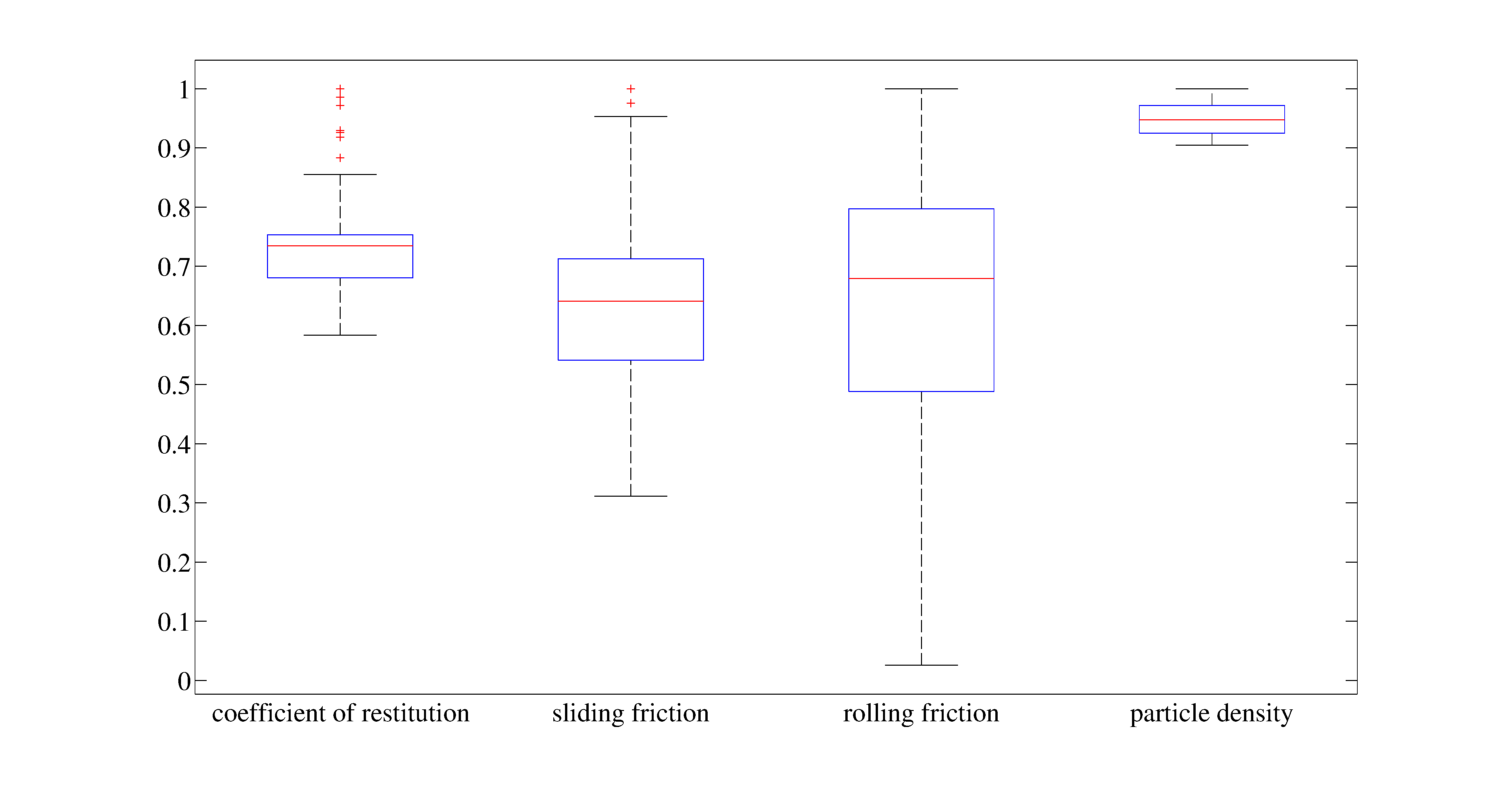
\includegraphics[width=.47\columnwidth]{images/166BoxSCTcokecoarsetest01coeffP1}
	  \label{fig:166BoxSCTcokecoarsetest01coeffP1}
  }
  \quad
  \subfloat[Density plot \acs{SCT}.]{
	  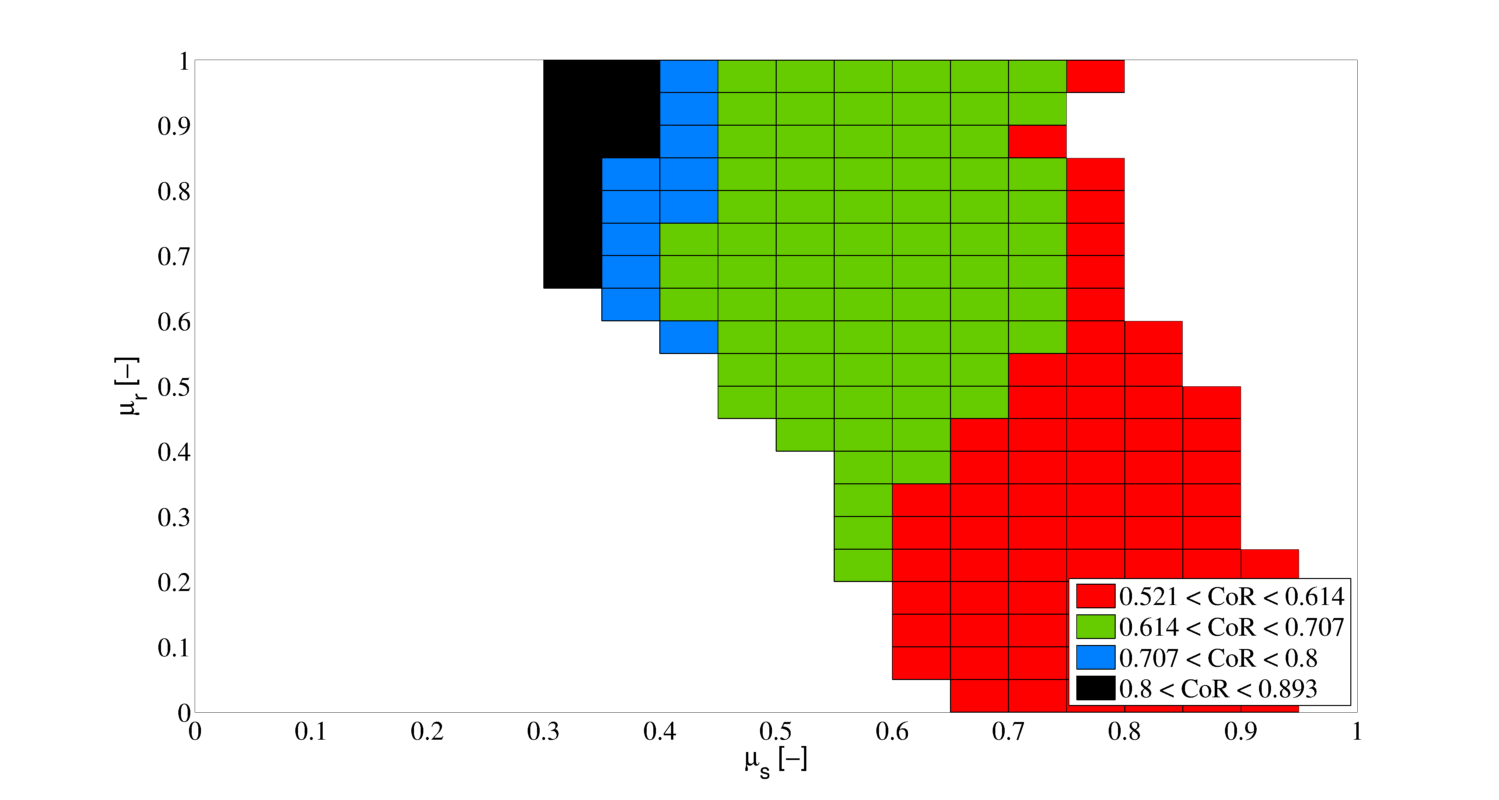
\includegraphics[width=.47\columnwidth]{images/172TileSCcokecoarsetest01coeffP1}
	  \label{fig:172TileSCcokecoarsetest01coeffP1}
  }
  \\
    \subfloat[Box plot \acs{AoR}.]{
	  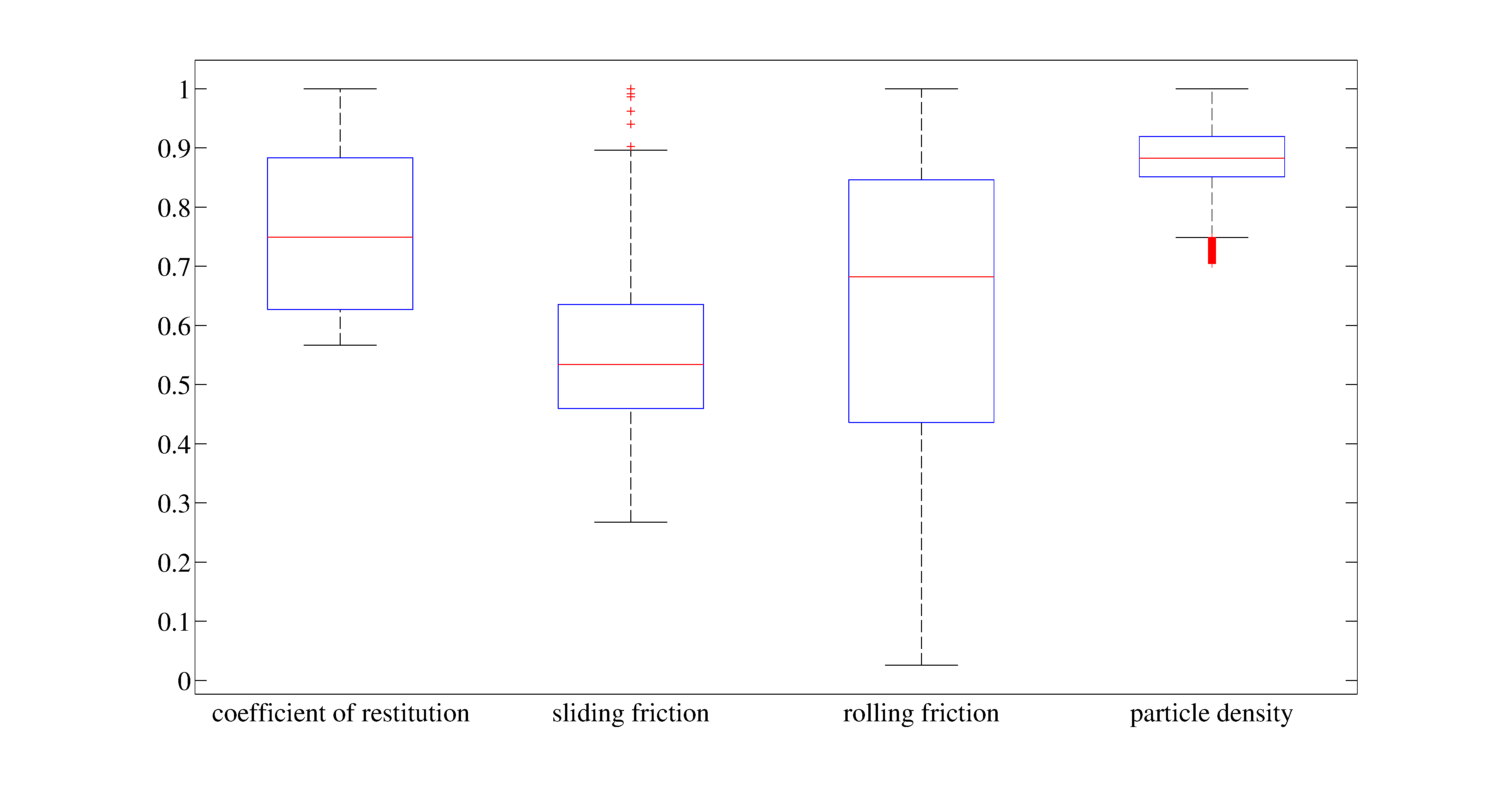
\includegraphics[width=.47\columnwidth]{images/177BoxAORcokecoarse}
	  \label{fig:177BoxAORcokecoarse}  }
  \quad
   \subfloat[Density plot \acs{AoR}.]{
	  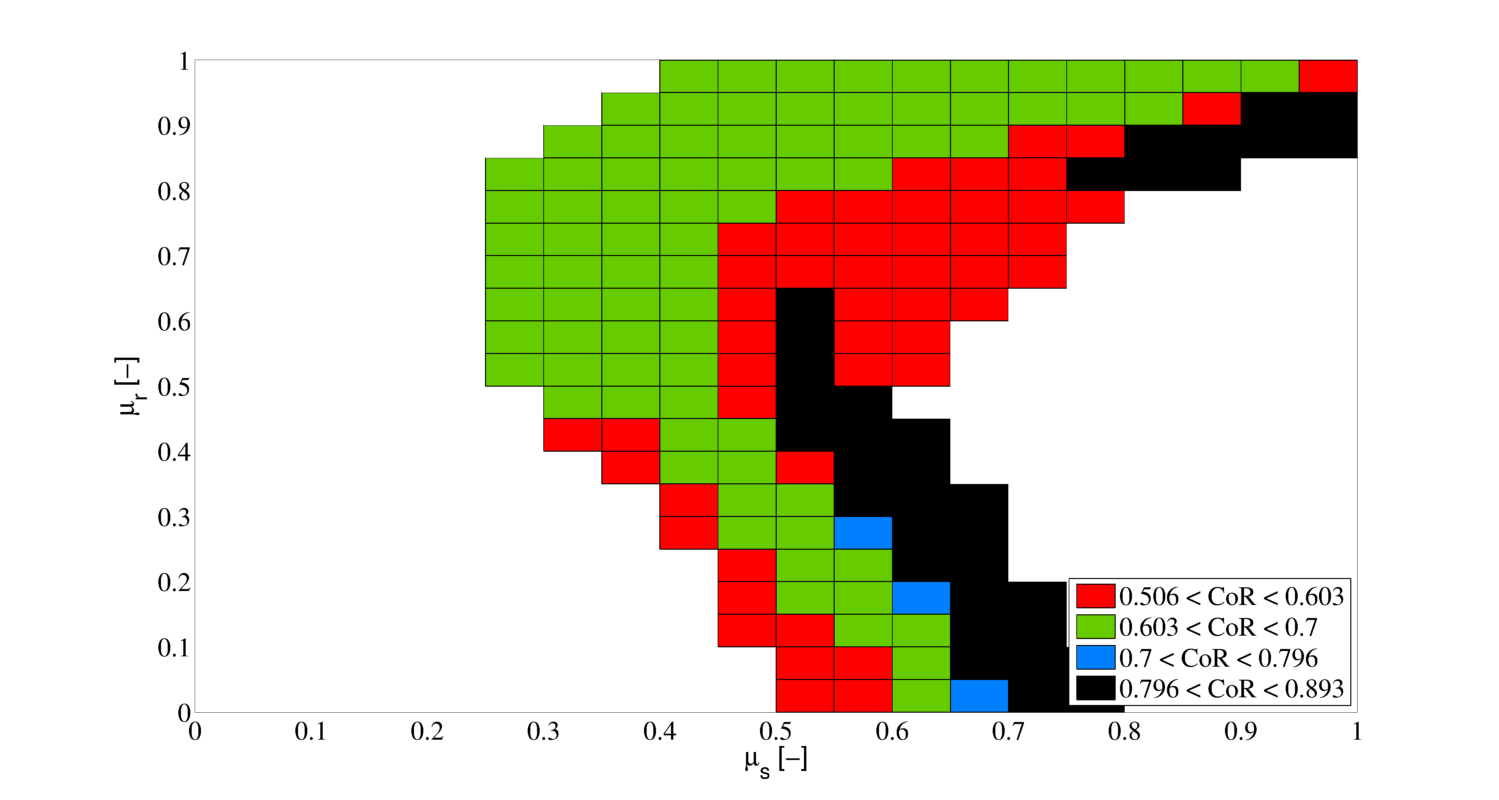
\includegraphics[width=.47\columnwidth]{images/178TileAORcokecoarse}
	  \label{fig:178TileAORcokecoarse}  }
  \\
  \subfloat[Box plot intersection: \acs{AoR} \& \acs{SCT}.]{
	  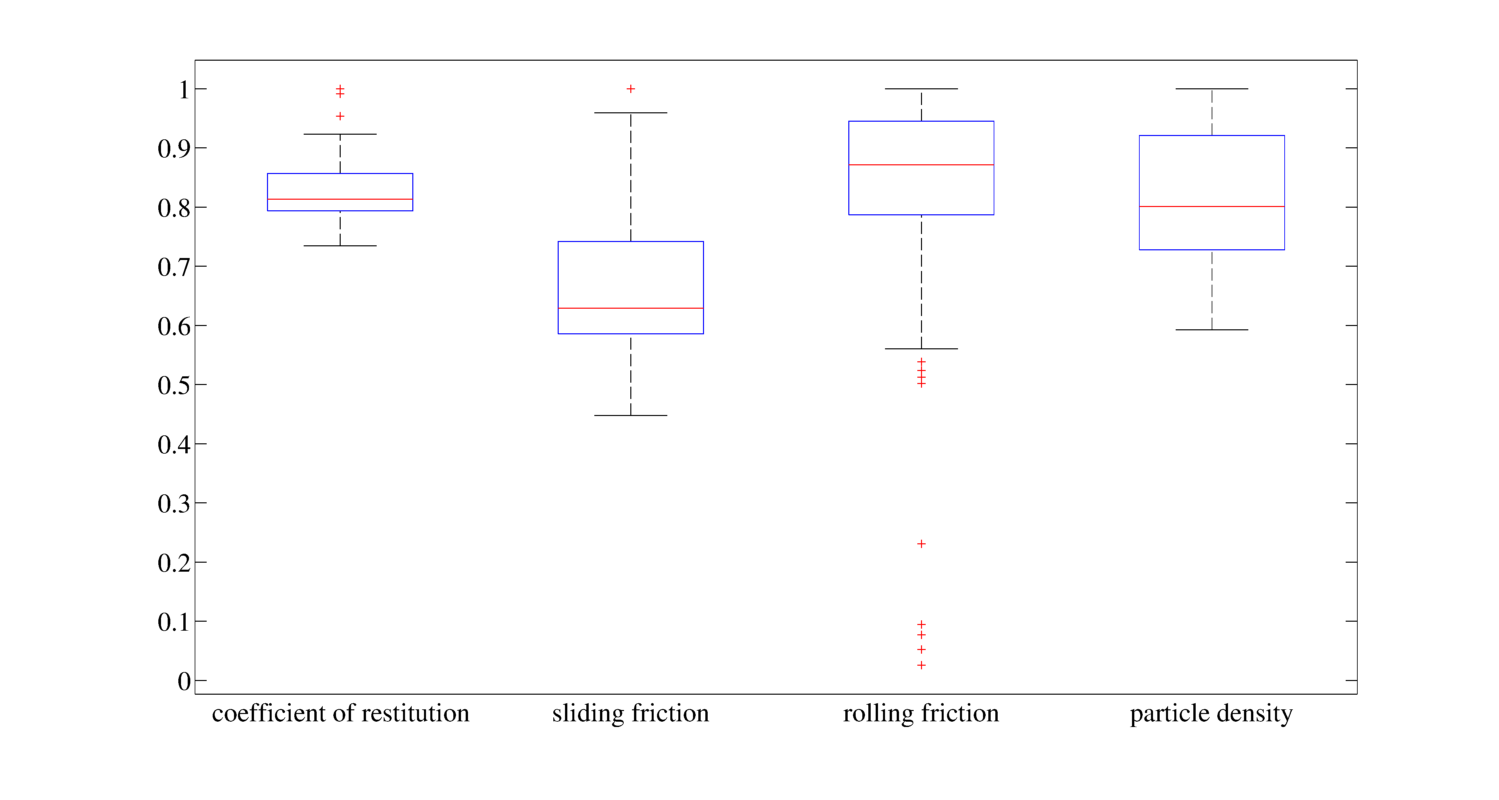
\includegraphics[width=.47\columnwidth]{images/197BoxMixcokecoarse_27}
	  \label{fig:197BoxMixcokecoarse_27}
  }
  \quad  
    \subfloat[Density plot intersection: \acs{AoR} \& \acs{SCT}.]{
	  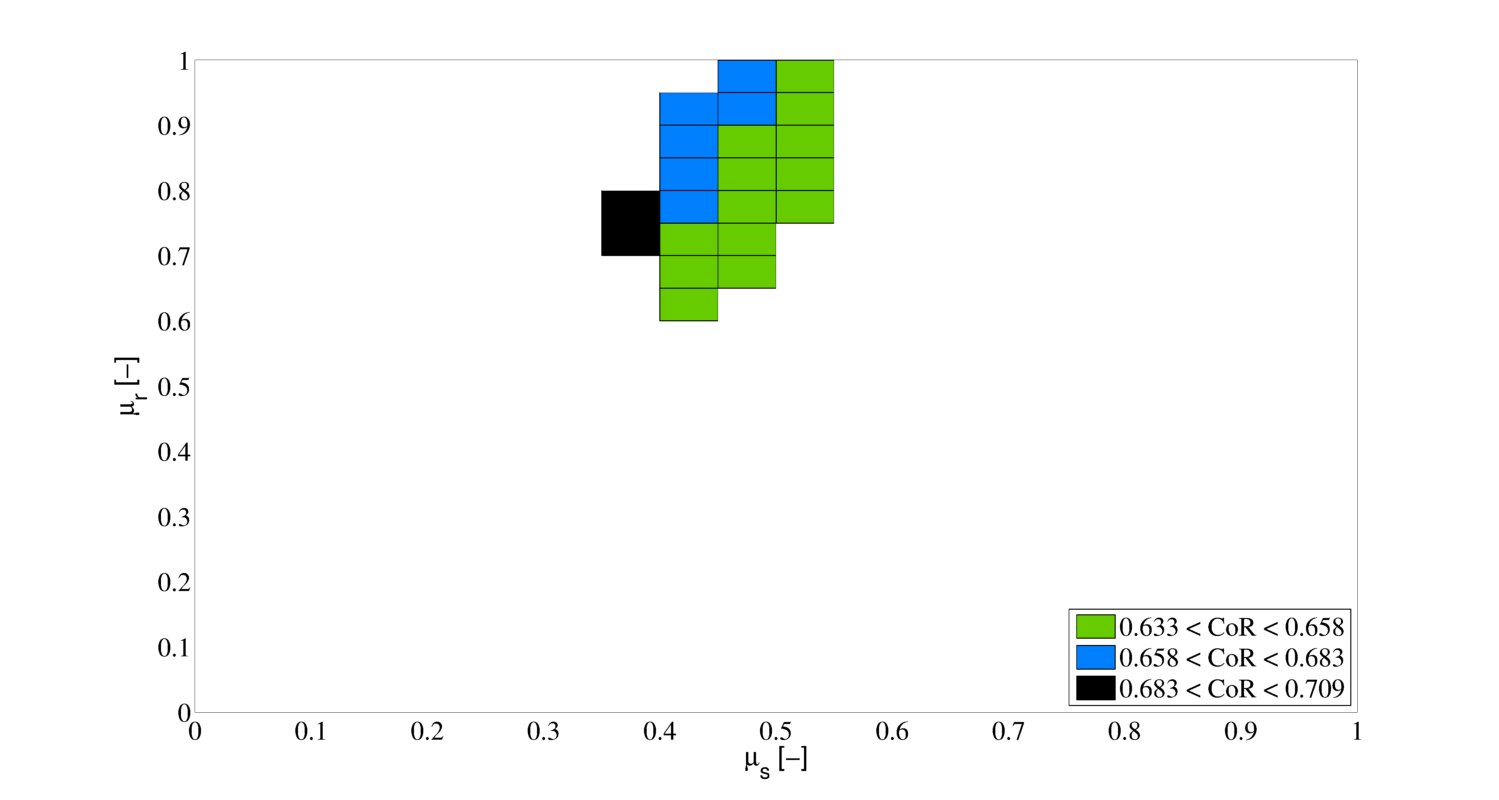
\includegraphics[width=.47\columnwidth]{images/198TileMixcokecoarse_27}
	  \label{fig:198TileMixcokecoarse_27}
  }
  \\    
  \caption[Coke coarse]{Coke coarse. The valid values for the \acs{SCT} and
  \acs{AoR} tests are shown, together with the merge values, valid for both.
  The plots referring to the single test show reasonably narrow confidence
  ranges, while Fig. \ref{fig:197BoxMixcokecoarse_27} shows unreasonably large
  valid ranges. See Section \ref{sec:remainingmaterialscharacterization} for
  the interpretation.}
  \label{fig:209boxplotscokecoarse}
\end{figure}